\documentclass{beamer}

\usepackage{hyperref}
\usepackage{pgfplots}
\usepackage{pgfplotstable}

\usetheme{UiO}

\hypersetup{
    colorlinks=true,
    urlcolor=blue
}

\title{Persontilpasset KI-basert nevrodiagnostikk}
\author{Esten H. Leonardsen}
\date{06.03.2024}

\titlegraphic{
	\centering
	\vspace{7.7cm}
	
\includegraphics[width=\logowidth]{data/uio_logo_full.png}
}

\usetikzlibrary{arrows}
\usetikzlibrary{arrows.meta}
\usetikzlibrary{calc}
\usetikzlibrary{fadings}
\usetikzlibrary{fillbetween}
\usetikzlibrary{patterns}
\usetikzlibrary{positioning}
\usetikzlibrary{shapes.arrows}

\newsavebox{\articles}
\sbox{\articles}{
    \begin{tikzpicture}
        \begin{axis}[
            height=6cm,
            width=9cm,
            xmin=1990,
            xmax=2024,
            xtick={1990, 1995, 2000, 2005, 2010, 2015, 2020},
            xticklabels={1990, 1995, 2000, 2005, 2010, 2015, 2020},
            xlabel={År},
            ymin=0,
            ymax=8000,
            ytick={2000, 4000, 6000},
            yticklabels={2000, 4000, 6000},
            ylabel={Antall publikasjoner},
            ylabel style={align=center, font=\small\linespread{0.9}\selectfont, yshift=0.4cm},
            xlabel style={font=\small},
            xtick pos=bottom,
            ytick pos=left,
            ticklabel style={font=\small},
            axis lines=left
        ]
            \addplot[
                cyan,
                very thick
            ] table[
                col sep=comma,
                x=Year,
                y=Count
            ] {data/PubMed_Timeline_Results_by_Year.csv};
        \end{axis}
    \end{tikzpicture}
}

\newsavebox{\dlperformance}
\sbox{\dlperformance}{
    \begin{tikzpicture}
        \begin{axis}[
            height=7cm,
            width=9cm,
            xmin=2012,
            xmax=2023,
            xlabel=År,
            ylabel={Treffsikkerhet (\%)},
            set layers,
            mark layer=axis tick labels,
            xtick pos=bottom,
            ytick pos=left,
            ymin=50,
            ymax=100,
            xtick={2013, 2015, 2017, 2019, 2021, 2023},
            xticklabels={2013, 2015, 2017, 2019, 2021, 2023},
            ytick={50, 60, 70, 80, 90, 100},
            yticklabels={50, 60, 70, 80, 90, 100}
        ]
            \addplot[
                only marks,
                mark=*,
                mark options={fill=cyan},
                mark size=3pt,
                opacity=0.25
            ] table [
                col sep=comma,
                x=year,
                y=accuracy
            ] {data/DL_accuracies.csv};

        \end{axis}
    \end{tikzpicture}
}

\begin{document}
	\begin{frame}
	 	\titlepage
	\end{frame}

    \newcommand{\mriside}[4]{
    \def\mridepth{0.75}

    \node[inner sep=0pt] (input) at (#1, #2) {
        \includegraphics[height=#3, width=#3]{#4}
    };

    \draw[fill=black] (input.north west) --
        ($ (input.north west) + (0.5 * \mridepth, 0.5 * \mridepth) $) --
        ($ (input.north east) + (0.5 * \mridepth, 0.5 * \mridepth) $) --
        (input.north east) -- cycle;
    \draw[fill=black] (input.north east) --
        ($ (input.north east) + (0.5 * \mridepth, 0.5 * \mridepth) $) --
        ($ (input.south east) + (0.5 * \mridepth, 0.5 * \mridepth) $) --
        (input.south east) -- cycle;
    \draw[] (input.north west) --
        ($ (input.north west) - (0.5 * \mridepth, 0.5 * \mridepth) $) --
        ($ (input.south west) - (0.5 * \mridepth, 0.5 * \mridepth) $) --
        (input.south west) -- cycle;
    \draw[] (input.north east) --
        ($ (input.north east) - (0.5 * \mridepth, 0.5 * \mridepth) $) --
        ($ (input.south east) - (0.5 * \mridepth, 0.5 * \mridepth) $) --
        (input.south east) -- cycle;
    \draw[] ($ (input.north west) - (0.5 * \mridepth, 0.5 * \mridepth) $) --
        ($ (input.north east) - (0.5 * \mridepth, 0.5 * \mridepth) $);
    \draw[] ($ (input.south west) - (0.5 * \mridepth, 0.5 * \mridepth) $) --
        ($ (input.south east) - (0.5 * \mridepth, 0.5 * \mridepth) $);
}


\newcommand{\inputside}[3]{
    \mriside{#1}{#2}{#3}{data/mri_sagittal.png}
}

\newcommand{\heatmapside}[3]{
    \mriside{#1}{#2}{#3}{data/combined_sagittal.png}
}

\newcommand{\convside}[6]{
    \def\sidex{#1}
    \def\sidey{#2}
    \def\sidewidth{#3}
    \def\sideheight{#4}
    \def\sidefillcolour{#5}
    \def\sidename{#6}

    \node[
        fill=\sidefillcolour,
        inner sep=0pt,
        outer sep=0pt,
        minimum width=\sidewidth,
        minimum height=\sideheight,
        draw=black
    ] (\sidename) at (\sidex, \sidey) {};
}

\newcommand{\convtop}[4]{
    \def\topbase{#1}
    \def\topwidth{#2}
    \def\topheight{#3}
    \def\topfillcolour{#4}

    \draw[fill=\topfillcolour,draw=black] #1 --
        ($ #1 + (#3, #3) $) --
        ($ #1 + (#3+#2, #3) $) --
        ($ #1 + (#2, 0) $);
}

\newcommand{\convfront}[3]{
    \def\frontbase{#1}
    \def\frontsize{#2}
    \def\frontfillcolour{#3}

    \draw[black, fill=\frontfillcolour] #1 --
        ($ #1 + (1*#2, 1*#2) $) --
        ($ #1 + (1*#2, 1*#2 - 2*#2) $) --
        ($ #1 + (0, -2*#2) $);
}

\newcommand{\convchannel}[7]{
    \def\channelx{#1}
    \def\channely{#2}
    \def\channelnodedepth{#3}
    \def\channelnodesize{#4}
    \def\channelnodecount{#5}
    \def\channelcolour{#6}
    \def\includefront{#7}

    \def\huemin{20}
    \def\huemax{80}

    \pgfmathsetmacro{\iterations}{#5-1}
    \foreach \i in {0,...,\iterations} {
        \pgfmathsetmacro{\hue}{int(random(\huemin, \huemax))}
        \convside{#1}{#2+\i*-#4}{#3 cm}{#4 cm}{#6!\hue}{n\i0}

        \foreach \j in {0,...,\iterations} {
            \pgfmathsetmacro{\innerhue}{int(random(\huemin, \huemax))}
            \ifnum\j=0
                \pgfmathsetmacro{\innerhue}{\hue}
            \fi

            \ifnum\includefront=1
                \convfront{($ (n00.north east) + (0.5*\j*#4, 0.5*\j*#4 - \i*#4) $)}{0.5*#4}{#6!\innerhue}
            \fi

            \ifnum\i=0
                \convtop{($ (n\i0.north west) + (0.5*\j*#4, 0.5*\j*#4) $)}{#3}{0.5*#4}{#6!\innerhue}
            \fi
        }
    }
}
\newcommand{\lrpchannel}[6]{
    \def\channelx{#1}
    \def\channely{#2}
    \def\channelnodedepth{#3}
    \def\channelnodesize{#4}
    \def\channelnodecount{#5}
    \def\includefront{#6}

    \colorlet{bgcolour}{black!85}

    \pgfmathsetmacro{\iterations}{#5-1}
    \foreach \i in {0,...,\iterations} {
        \pgfmathsetmacro{\hue}{int(random(-150, 100))}
        \colorlet{fillcolour}{bgcolour}

        \colorlet{lrpcolour}{red}
        \pgfmathsetmacro{\coinflip}{int(random(0, 1))}

        \ifnum\coinflip=1
            \colorlet{lrpcolour}{blue}
        \fi

        \ifnum\hue>0
            \colorlet{fillcolour}{lrpcolour!\hue!bgcolour}
        \fi

        \convside{#1}{#2+\i*-#4}{#3 cm}{#4 cm}{fillcolour}{n\i0}

        \foreach \j in {0,...,\iterations} {
            \pgfmathsetmacro{\innerhue}{int(random(-150, 100))}
            \colorlet{innerfillcolour}{bgcolour}

            \ifnum\innerhue>0
                \colorlet{innerfillcolour}{lrpcolour!\innerhue!bgcolour}
            \fi

            \ifnum\j=0
                \colorlet{innerfillcolour}{fillcolour}
            \fi

            \ifnum\includefront=1
                \convfront{($ (n00.north east) + (0.5*\j*#4, 0.5*\j*#4 - \i*#4) $)}{0.5*#4}{innerfillcolour}
            \fi

            \ifnum\i=0
                \convtop{($ (n\i0.north west) + (0.5*\j*#4, 0.5*\j*#4) $)}{#3}{0.5*#4}{innerfillcolour}
            \fi
        }
    }
}


\newcommand{\convlayer}[7]{
    \def\layerx{#1}
    \def\layery{#2}
    \def\layernodedepth{#3}
    \def\layernodesize{#4}
    \def\layernodecount{#5}
    \def\layerdepth{#6}
    \def\layercolour{#7}

    \pgfmathsetmacro{\layeriterations}{\layerdepth-1}
    \foreach \i in {0,...,\layeriterations}{
        \pgfmathsetmacro{\x}{\layerx + \i * \layernodedepth}
        \pgfmathsetmacro{\islast}{\i == \layeriterations ? 1 : 0}
        \convchannel{\x}{\layery}{\layernodedepth}{\layernodesize}{\layernodecount}{\layercolour}{\islast}
    }
}
\newcommand{\lrplayer}[6]{
    \def\layerx{#1}
    \def\layery{#2}
    \def\layernodedepth{#3}
    \def\layernodesize{#4}
    \def\layernodecount{#5}
    \def\layerdepth{#6}

    \pgfmathsetmacro{\layeriterations}{\layerdepth-1}
    \foreach \i in {0,...,\layeriterations}{
        \pgfmathsetmacro{\x}{\layerx + \i * \layernodedepth}
        \pgfmathsetmacro{\islast}{\i == \layeriterations ? 1 : 0}
        \lrpchannel{\x}{\layery}{\layernodedepth}{\layernodesize}{\layernodecount}{\islast}
    }
}

\newcommand{\modelarrow}[5]{
    \begin{scope}[transparency group, opacity=0.5]
        \draw[-stealth, line width=2pt, #3] #1 to [in=#4, out=#5] #2;
    \end{scope}
}
\newcommand{\cnnarrow}[3]{
    \modelarrow{#1}{#2}{#3}{180}{0}
}
\newcommand{\lrparrow}[3]{
    \modelarrow{#1}{#2}{#3}{0}{180}
}

\newcommand{\cnn}[6]{
    \def\xmin{#1}
    \def\ymin{#2}
    \def\nodedepth{#3}
    \def\nodesize{#4}
    \def\modelcolour{#5}
    \def\annotate{#6}

    \convlayer{#1 - 0.06 + 0.4}{#2 + 2.5 * #4}{#3}{#4}{12}{3}{\modelcolour}
    \cnnarrow{(#1 + 1.04, #2)}{(#1+2.2, #2)}{black}

    \convlayer{#1 + 1.44 + 0.4}{#2 + 1.5 * #4}{#3}{#4}{8}{5}{\modelcolour}
    \cnnarrow{(#1 + 2.59, #2)}{(#1+3.5, #2)}{black}

    \convlayer{#1 + 2.77 + 0.4}{#2 + 0.5 * #4}{#3}{#4}{4}{7}{\modelcolour}
    \cnnarrow{(#1 + 3.98, #2)}{(#1+5, #2)}{black}

    \convlayer{#1 + 3.93 + 0.4}{#2 + 0}{#3}{#4}{2}{9}{\modelcolour}

    \draw[thick, dashed] (#1 + 0.22, #2 + 1.43) --
                        (#1 + 5.4, #2 + 1.43) --
                        (#1 + 5.4, #2 - 1.42) --
                        (#1 + 0.22, #2 - 1.42) -- cycle;
    \node[anchor=south, text depth=0, font=\footnotesize\selectfont] at (#1 + 2.675, #2 + 1.43) {
        \textbf{Convolutional neural network}
    };
}
\newcommand{\lrp}[4]{
    \def\xmin{#1}
    \def\ymin{#2}
    \def\nodedepth{#3}
    \def\nodesize{#4}

    \lrplayer{#1 - 0.06 + 0.4}{#2 + 2.5 * #4}{#3}{#4}{12}{3}{black}
    \lrparrow{(#1+2.2, #2)}{(#1 + 1.04, #2)}{black}

    \lrplayer{#1 + 1.44 + 0.4}{#2 + 1.5 * #4}{#3}{#4}{8}{5}{black}
    \lrparrow{(#1+3.5, #2)}{(#1 + 2.59, #2)}{black}

    \lrplayer{#1 + 2.77 + 0.4}{#2 + 0.5 * #4}{#3}{#4}{4}{7}{black}
    \lrparrow{(#1+5, #2)}{(#1 + 3.98, #2)}{black}

    \lrplayer{#1 + 3.93 + 0.4}{#2 + 0}{#3}{#4}{2}{9}{black}

    \draw[thick, dashed] (#1 + 0.22, #2 + 1.43) --
                        (#1 + 5.4, #2 + 1.43) --
                        (#1 + 5.4, #2 - 1.42) --
                        (#1 + 0.22, #2 - 1.42) -- cycle;
    \node[anchor=south, text depth=0, font=\footnotesize\selectfont] at (#1 + 2.675, #2 + 1.43) {
        \textbf{Convolutional Neural Network}
    };
}

    \begin{frame}{KI-revolusjonen(?)}
        \begin{tikzpicture}
            \node[] at (-5.25, 3.5) {};
            \node[] at (5.25, -3.5) {};

            \only<1>{
                \node[inner sep=0pt, draw=black] at (0, 0) {
                    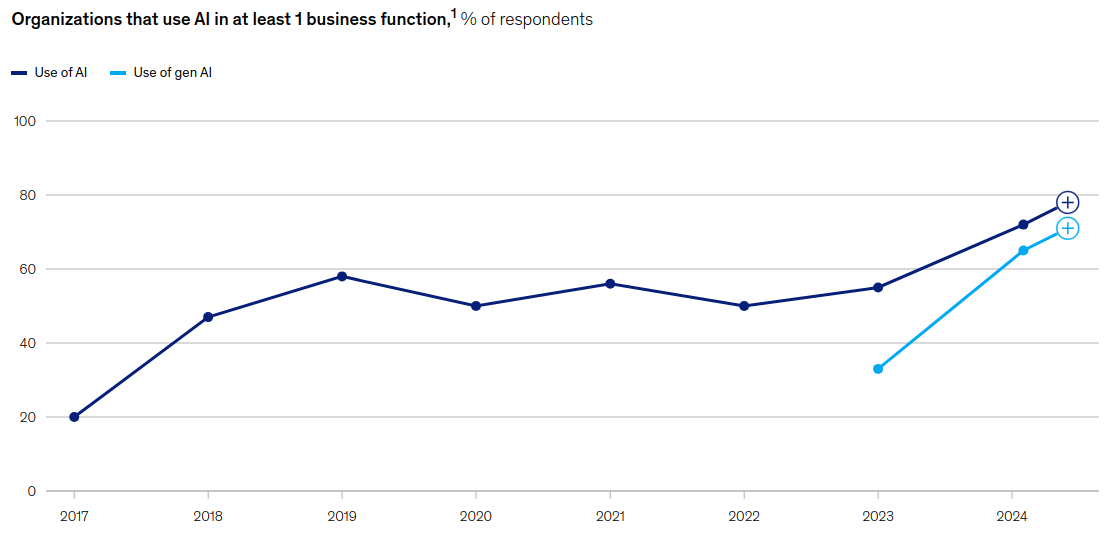
\includegraphics[width=9cm]{data/mckinsey.png}
                };
                \node[anchor=south, font=\tiny, text width=10cm, align=flush center] at (0, -3.75) {
                    McKinsey \& Company, The state of AI: How organizations are rewiring to capture value, \textit{https://www.mckinsey.com/capabilities/quantumblack/our-insights/the-state-of-ai} (2025)
                };
            }
            \only<2>{
                \node[] at (0, 0) {
                    \usebox{\articles}
                };
                \node[anchor=south, font=\tiny, text width=10cm, align=flush center] at (0, -3.75) {
                    https://pubmed.ncbi.nlm.nih.gov/, publikasjoner som inneholder "(neurology OR neuroscience OR neuroimaging) AND (ai OR artificial intelligence OR deep learning)"
                };
            }
            \only<3>{
                \node[] at (0, 0) {
                    \usebox{\cnntraining}
                };
                \node[anchor=south, font=\tiny, text width=10cm, align=flush center] at (0, -3.75) {
                    Leonardsen, E. H., ... \& Wang, Y. (2024). Constructing personalized characterizations of structural brain aberrations in patients with dementia using explainable artificial intelligence. \textit{NPJ Digital Medicine}, 7(1), 110
                };
            }
            \only<4>{
                \node[] at (0, 0) {
                    \usebox{\dlperformance}
                };
            }
            \only<5>{
                \node[text width=9cm, align=flush center] at (0, 0) {
                    "Innføringen av KI i helse- og omsorgstjenesten har gått saktere enn noen forventet i starten av planperioden"
                };
                \node[anchor=south, font=\tiny, text width=10cm, align=flush center] at (0, -3.75) {
                    Helsedirektoratet (2023). Status og forslag til videre arbeid med kunstig intelligens (KI) i helse- og omsorgstjenesten. Oslo: Helsedirektoratet (siste faglige endring 26. oktober 2023). Tilgjengelig fra https://www.helsedirektoratet.no/rapporter/status-og-forslag-til-videre-arbeid-med-kunstig-intelligens-ki-i-helse-og-omsorgstjenesten
                };
            }
        \end{tikzpicture}
    \end{frame}

    \begin{frame}{Utfordringer: Forklarbarhet}
        \begin{tikzpicture}
            \node[] at (-5.25, 3.5) {};
            \node[] at (5.25, -3.5) {};

            \only<1>{
                \node[] at (0, 0) {
                    \usebox{\cnntraining}
                };
            }

            \only<2>{
                \node[] at (0, 0) {
                    \usebox{\cnnheatmap}
                };
            }
            \only<3-4>{
                \node[inner sep=0pt, label=above:{Kunstig intelligens}] at (-2.5, 0) {
                    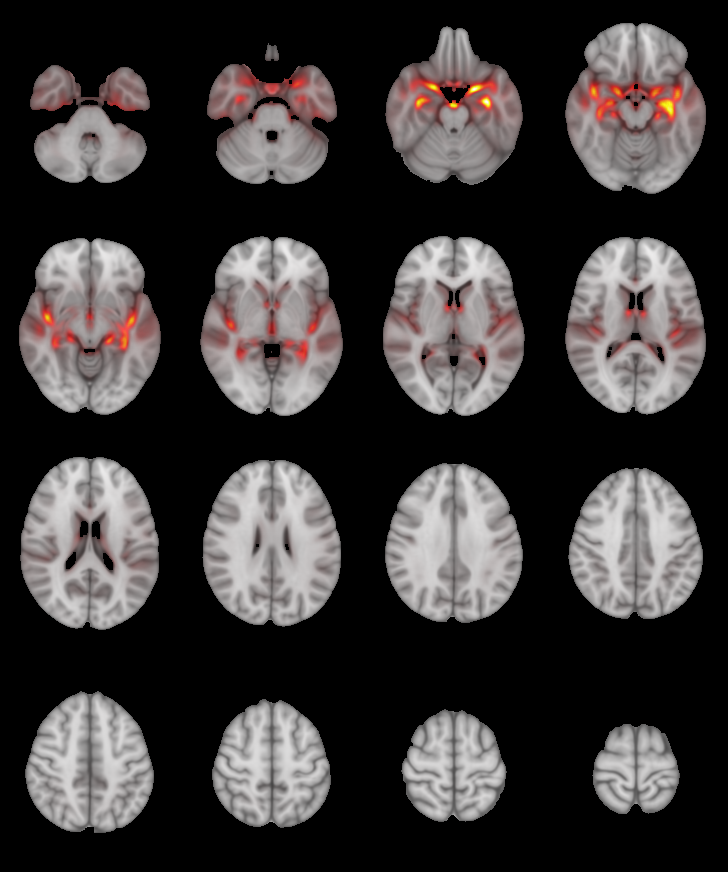
\includegraphics[width=4cm]{data/dementia_average.png}
                };
            }
            \only<4>{
                \node[inner sep=0pt, label=above:{Menneskelige forskere}] at (2.5, 0) {
                    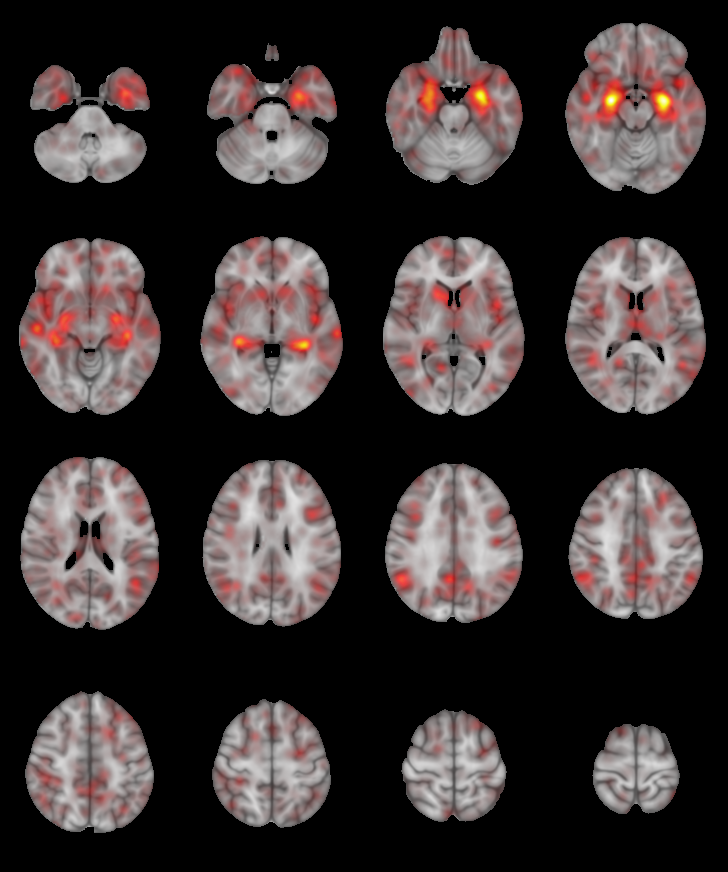
\includegraphics[width=4cm]{data/ALE.png}
                };
            }
        \end{tikzpicture}
    \end{frame}

    \begin{frame}{Utfordringer: Nytteverdi}
        \begin{tikzpicture}
            \node[] at (-5.25, 3.25) {};
            \node[] at (5.25, -3.25) {};

            \only<1>{
                \node[] at (0, 0) {
                    \usebox{\cnntraining}
                };
            }
            \node[
                minimum height=0.72cm,
                minimum width=2.02cm,
                thick,
                draw=red
            ] at (4.06, -0.25) {};
        \end{tikzpicture}
    \end{frame}

    \begin{frame}{baba.vision}
        \begin{tikzpicture}
            \node[] at (-5.25, 3.25) {};
            \node[] at (5.25, -3.25) {};

            \only<1>{
                \node[] at (0, 0) {
                    
\includegraphics[width=7cm]{data/babatext.png}
                };
            }
            \only<2>{
                \node[] at (0, 0) {
                    baba team
                };
            }
            \only<3>{
                \node[text width=10cm, align=center] at (0, 0) {
                    \href{https://mlflow-server-531474577141.us-central1.run.app/\#/experiments/0}{https://mlflow-server-531474577141.us-central1.run.app/\#/experiments/0}
                };
            }
        \end{tikzpicture}
    \end{frame}

    \newcommand{\stickman}[2]{
        \node[circle,fill,minimum size=2.5mm,#2] (head) at #1 {};
        \node[rounded corners=1pt,minimum height=0.65cm,minimum width=0.2cm,fill,below = 0.5pt of head,#2] (body) {};
        \draw[line width=0.5mm,round cap-round cap,#2] ([shift={(1pt,-0.5pt)}]body.north east) --++(-90:3mm);
        \draw[line width=0.5mm,round cap-round cap,#2] ([shift={(-1pt,-0.5pt)}]body.north west)--++(-90:3mm);
        \draw[thick,white,-round cap] (body.south) --++(90:2.75mm);
    }

    \newcommand{\response}[1]{
        \begin{tikzpicture}
            \node[] at (-4, -3) {};
            \node[] at (4, 3) {};

            \ifnum#1=0
                \draw[densely dotted, thick] (-3.75, -0.8) -- (3.75, -0.8);
                \node[anchor=south east, font=\tiny, inner sep=1pt] at (3.75, -0.8) {Eksklusjonskriterie};
                \draw[densely dotted, thick] (-0.7, -2.75) -- (-0.7, 3.1);
                \node[anchor=south east, font=\tiny, inner sep=1pt, rotate=90] at (-0.7, 3.1) {Eksklusjonskriterie};
            \fi

            \ifnum#1=1
                \draw[densely dotted, thick, blue!87!red] plot [smooth] coordinates {(-3.75, -0.5) (-1.1, -1.1) (0, -2.75)};
                \draw[densely dotted, thick, blue!62!red] plot [smooth] coordinates {(-3.75, 0.5) (-0.5, -0.95) (1.7, -2.75)};
                \draw[densely dotted, thick, blue!37!red] plot [smooth] coordinates {(-3.75, 2.75) (-1.25, 0.5) (3.75, -1.1)};
                \draw[densely dotted, thick, blue!12!red] plot [smooth] coordinates {(-0.3, 3.1) (0.6, 1) (3.75, 0.8)};
            \fi

            \node [
                single arrow,
                left color=blue,
                right color=red,
                single arrow head extend=3pt,
                transform shape,
                minimum height=1.5cm,
                text width=7cm,
                text=white,
                align=center,
                font=\footnotesize\bfseries
            ] at (0, -2.75) {Nevrologiske risikofaktorer};
            \node [
                single arrow,
                bottom color=blue,
                top color=red,
                single arrow head extend=3pt,
                transform shape,
                minimum height=1.5cm,
                text width=5.814cm,
                text=white,
                align=center,
                rotate=90,
                font=\footnotesize\bfseries
            ] at (-3.75, 0) {Genetiske risikofaktorer};

            \ifnum#1=0
                \stickman{(-3, -1.5)}{blue}
                \stickman{(-2.5, -1.4)}{blue}
                \stickman{(-3.1, -0.3)}{blue}
                \stickman{(-2.55, -0.25)}{blue}
                \stickman{(-2, -0.7)}{blue}
                \stickman{(-1.5, -1.1)}{blue}
                \stickman{(-2.8, 0.8)}{red}
                \stickman{(-2.1, 0.5)}{red}
                \stickman{(-1.5, 0.1)}{red}
                \stickman{(-0.95, -1.45)}{blue}
                \stickman{(-0.95, 0.3)}{red}
                \stickman{(-0.3, -0.7)}{red}
                \stickman{(-2.95, 2)}{red}
                \stickman{(-2.4, 1.8)}{red}
                \stickman{(-1.9, 2.7)}{red}
                \stickman{(-1.75, 1.5)}{red}
                \stickman{(-1.2, 1.65)}{red}
                \stickman{(-0.45, 0.7)}{red}
                \stickman{(0.1, 0)}{red}
                \stickman{(0.2, -1.1)}{red}
                \stickman{(0.3, 1.2)}{red}
                \stickman{(-0.3, 2.1)}{red}
                \stickman{(0.85, 2.4)}{red}
                \stickman{(1.1, 1.05)}{red}
                \stickman{(0.6, 0.2)}{red}
                \stickman{(0.7, -1.35)}{red}
                \stickman{(1.05, -0.6)}{red}
                \stickman{(1.65, -1.5)}{red}
                \stickman{(1.5, -0.2)}{red}
                \stickman{(1.5, 2)}{red}
                \stickman{(1.8, 0.95)}{red}
                \stickman{(2.2, 2.1)}{red}
                \stickman{(2.15, -1.1)}{red}
                \stickman{(2.8, -1.45)}{red}
                \stickman{(2.55, 0.6)}{red}
                \stickman{(3.15, 1.1)}{red}
                \stickman{(2.9, 2.45)}{red}
            \fi
            \ifnum#1=1
                \stickman{(-3, -1.5)}{blue}
                \stickman{(-2.5, -1.4)}{blue}
                \stickman{(-3.1, -0.3)}{blue}
                \stickman{(-2.55, -0.25)}{blue}
                \stickman{(-2, -0.7)}{blue}
                \stickman{(-1.5, -1.1)}{blue}
                \stickman{(-0.95, -1.45)}{blue}
                \stickman{(-2.8, 0.8)}{blue!75!red}
                \stickman{(-2.1, 0.5)}{blue!75!red}
                \stickman{(-1.5, 0.1)}{blue!75!red}
                \stickman{(-0.3, -0.7)}{blue!75!red}
                \stickman{(0.2, -1.1)}{blue!75!red}
                \stickman{(0.7, -1.35)}{blue!75!red}
                \stickman{(-0.95, 0.3)}{blue!50!red}
                \stickman{(-2.95, 2)}{blue!50!red}
                \stickman{(-2.4, 1.8)}{blue!50!red}
                \stickman{(-1.75, 1.5)}{blue!50!red}
                \stickman{(-0.45, 0.7)}{blue!50!red}
                \stickman{(0.1, 0)}{blue!50!red}
                \stickman{(0.6, 0.2)}{blue!50!red}
                \stickman{(1.05, -0.6)}{blue!50!red}
                \stickman{(1.65, -1.5)}{blue!50!red}
                \stickman{(1.5, -0.2)}{blue!50!red}
                \stickman{(2.15, -1.1)}{blue!50!red}
                \stickman{(2.8, -1.45)}{blue!50!red}
                \stickman{(-1.9, 2.7)}{blue!25!red}
                \stickman{(-1.2, 1.65)}{blue!25!red}
                \stickman{(0.3, 1.2)}{blue!25!red}
                \stickman{(-0.3, 2.1)}{blue!25!red}
                \stickman{(1.1, 1.05)}{blue!25!red}
                \stickman{(1.8, 0.95)}{blue!25!red}
                \stickman{(0.85, 2.4)}{blue!0!red}
                \stickman{(1.5, 2)}{blue!0!red}
                \stickman{(2.2, 2.1)}{red}
                \stickman{(2.55, 0.6)}{blue!25!red}
                \stickman{(3.15, 1.1)}{blue!25!red}
                \stickman{(2.9, 2.45)}{red}
            \fi
        \end{tikzpicture}
    }

    \begin{frame}{Prediksjon av behandlingsrespons}
        \begin{tikzpicture}
            \node[] at (-5.25, 3.5) {};
            \node[] at (5.25, -3.5) {};

            \only<1>{
                \node[inner sep=0pt, draw=black] at (0, 0) {
                    
\includegraphics[width=6cm]{data/ema.png}
                };
            }
            \only<2>{
                \node[inner sep=0pt, draw=black] at (0, 0) {
                    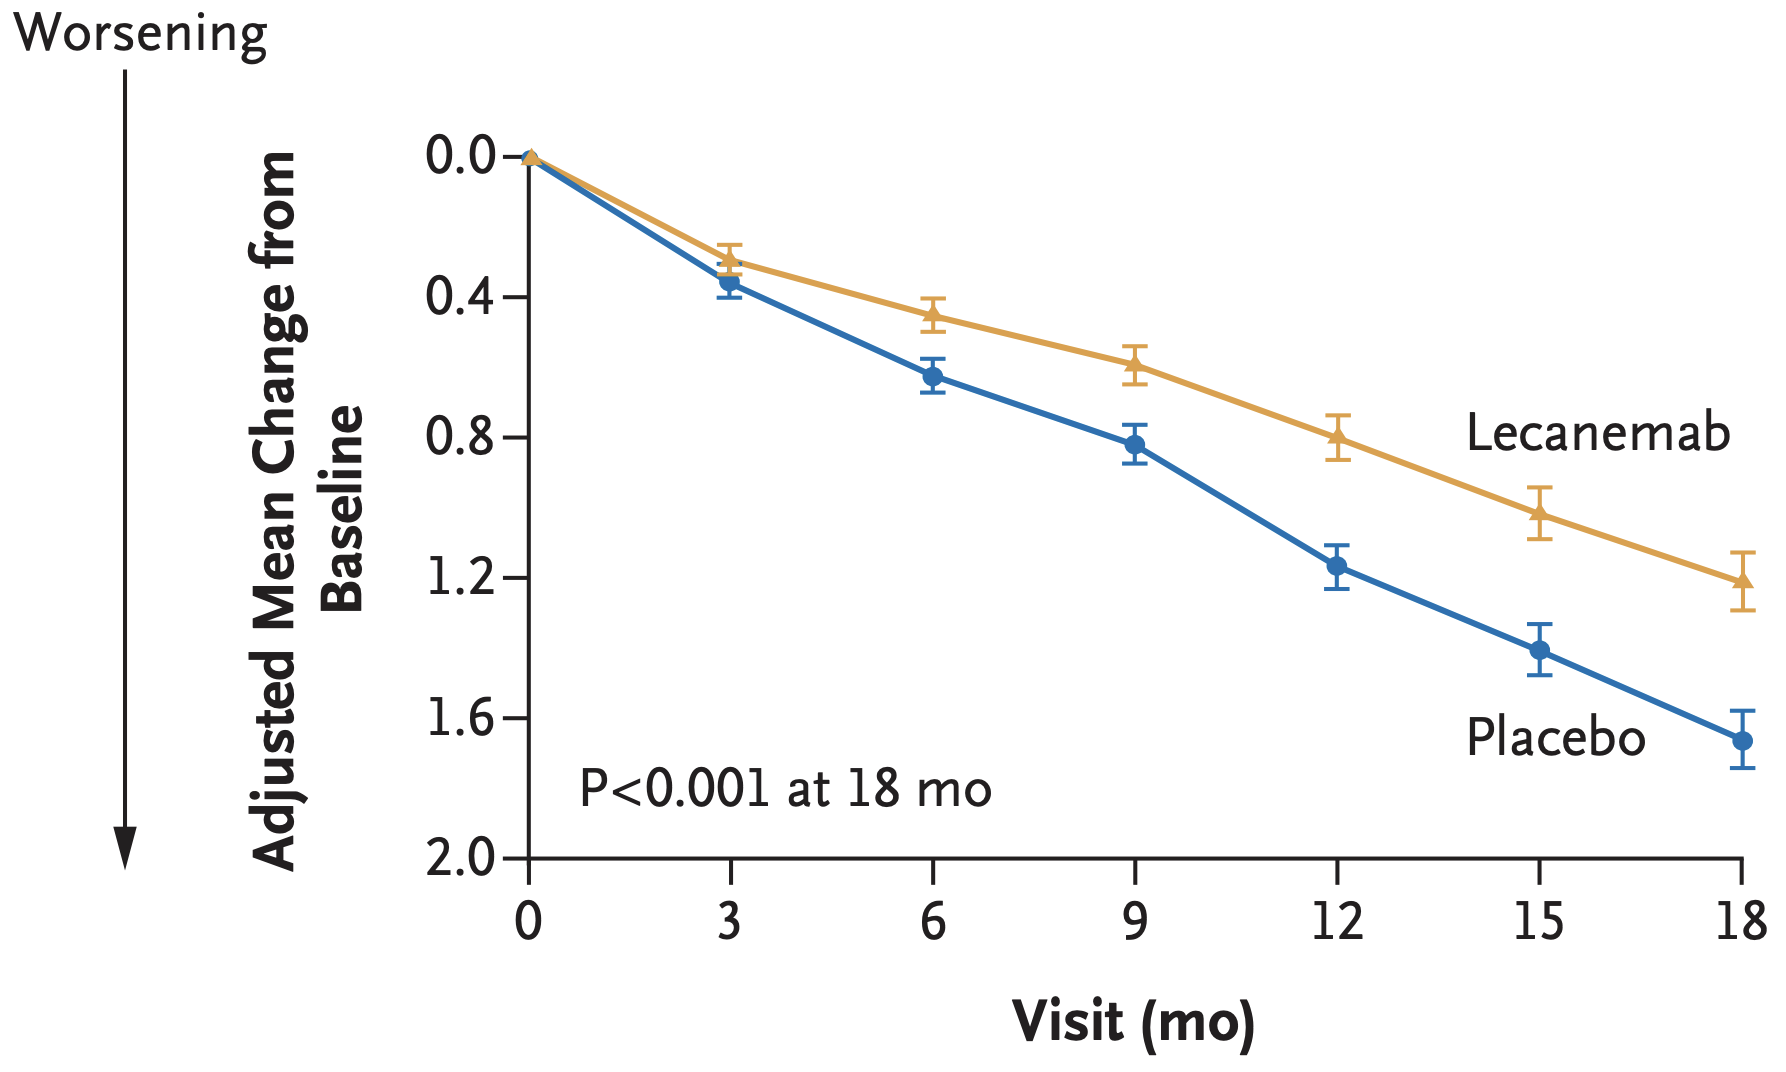
\includegraphics[width=8.5cm]{data/worsening.png}
                };
                \node[anchor=south, font=\tiny, text width=10cm, align=flush center] at (0, -3.75) {
                    Van Dyck, C. H., Swanson, C. J., Aisen, P., Bateman, R. J., Chen, C., Gee, M., ... \& Iwatsubo, T. (2023). Lecanemab in early Alzheimer’s disease. \textit{New England Journal of Medicine}.
                };
            }
            \only<3>{
                \node[] at (0, 0) {
                    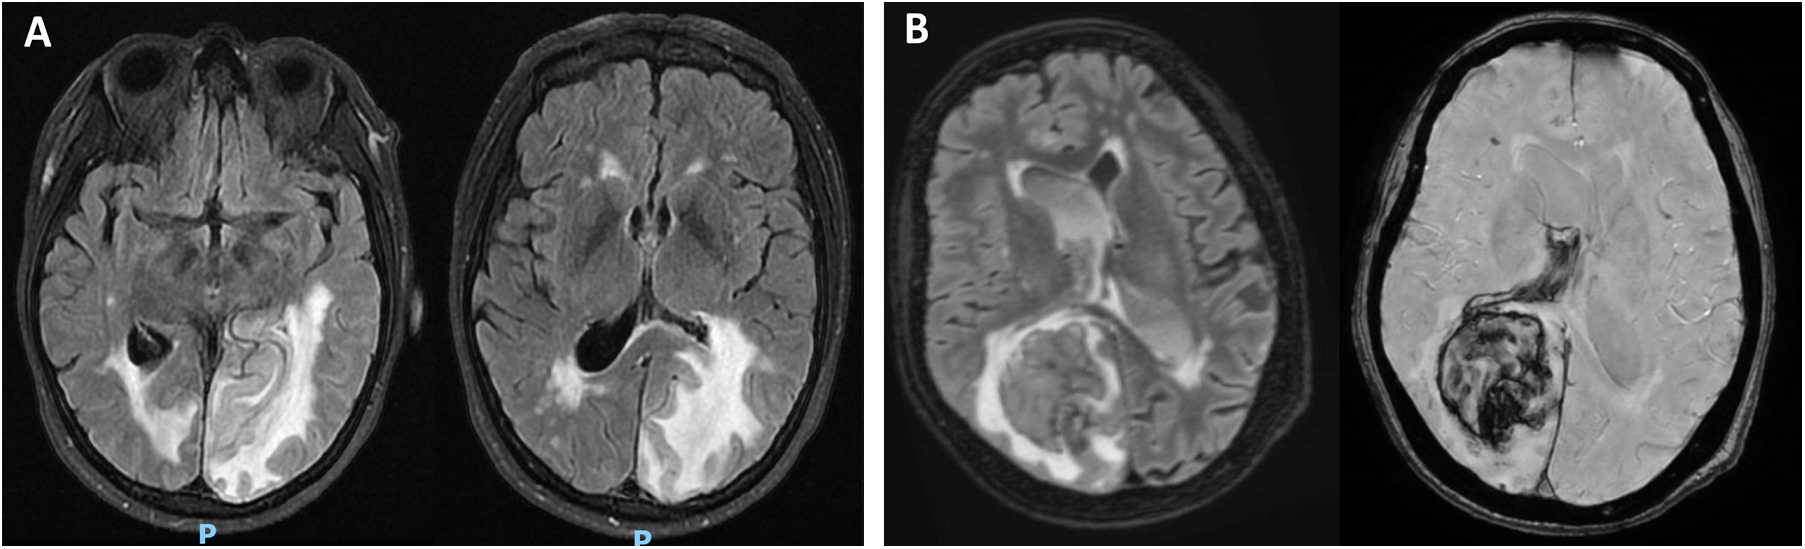
\includegraphics[width=10cm]{data/aria.jpg}
                };
                \node[anchor=south, font=\tiny, text width=10cm, align=flush center] at (0, -3.75) {
                    Villain, N., Planche, V., \& Levy, R. (2022). High-clearance anti-amyloid immunotherapies in Alzheimer's disease. Part 1: Meta-analysis and review of efficacy and safety data, and medico-economical aspects. \textit{Revue neurologique}.
                };
            }
            \visible<4>{
                \node[] at (0, 0) {
                    \response{0}
                };
            }
            \visible<5>{
                \node[] at (0, 0) {
                    \response{1}
                };
            }
            \only<6>{
                \node[] at (0, 0) {
                    feasbility study
                };
            }
            \only<7>{
                \node[inner sep=0pt, draw=black] at (0, 0) {
                    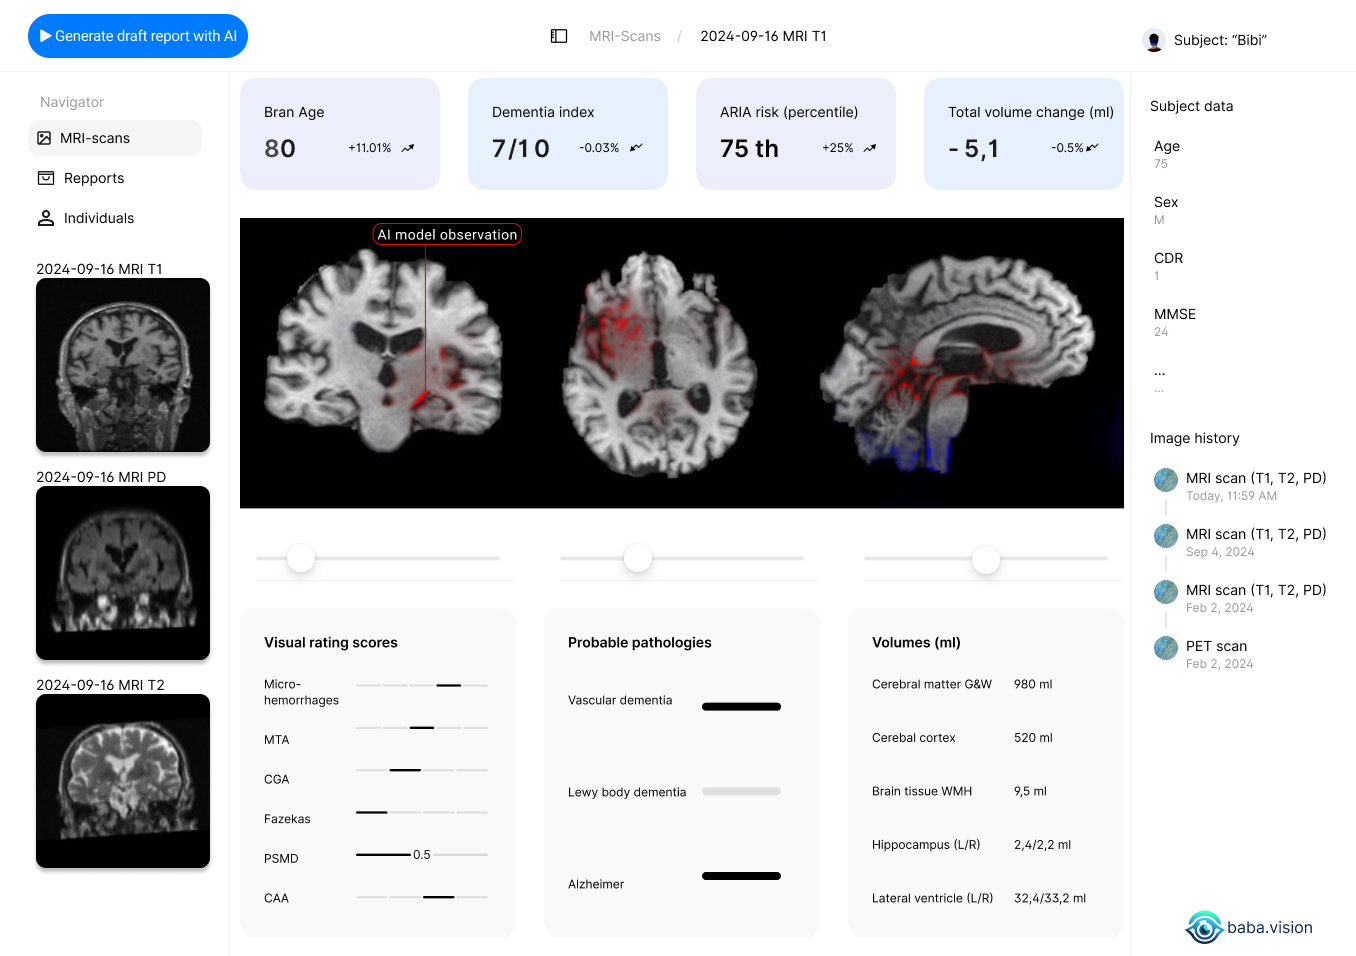
\includegraphics[width=8cm]{data/prototype.png}
                };
            }
        \end{tikzpicture}
    \end{frame}
\end{document}
